    \chapter{Anexo referente às imagens dos gráficos utilizados no relatório (TripAdvisor-Actividades)}
    \label{an3}

    Acesso a todos os gráficos originados: \href{https://github.com/CatKinKitKat/pi2021/tree/master/projecto/datascience/graphs/TripAdvisor/activities}{GitHub}.
    
    \begin{figure}[!htb]
    \centering
    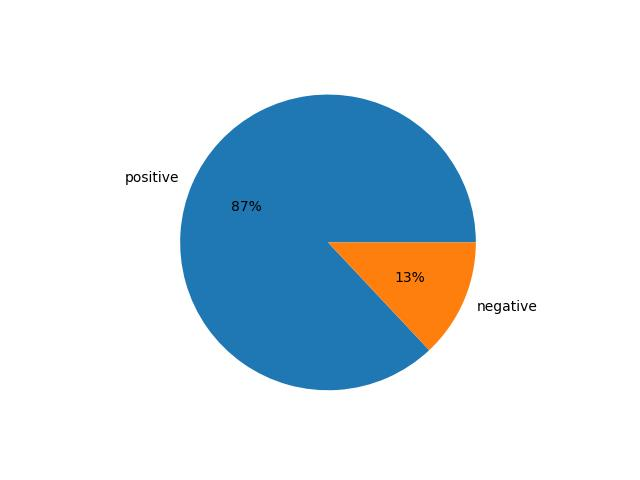
\includegraphics[width=7cm]{figuras/TripAdvisor/Activities/place0_sentiments.jpeg}
    \caption{Gráfico circular gerado baseando-se nos \textit{sentiments} mais usados da plataforma \textit{TripAdvisor} referente ao Castelo de Beja}
    \label{fig:exemplofig}
    \end{figure}
    
    \begin{figure}[!htb]
    \centering
    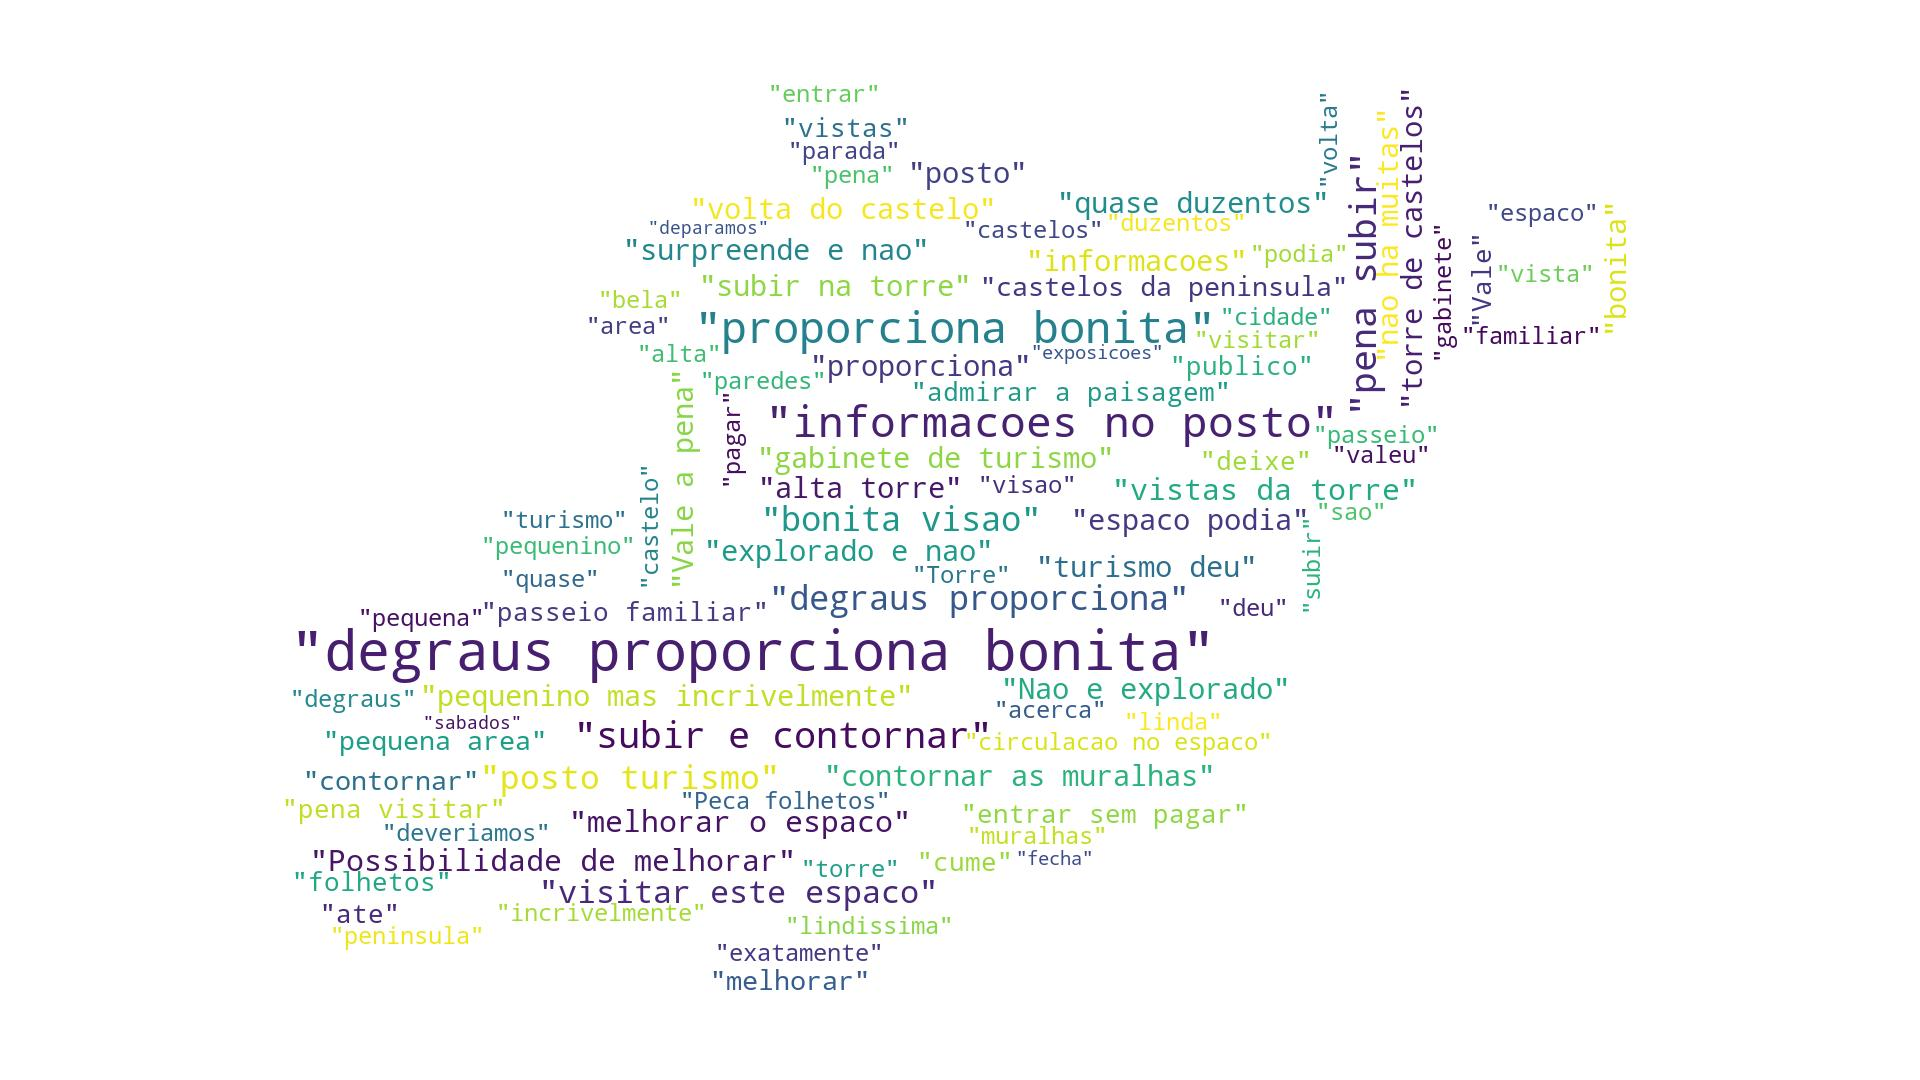
\includegraphics[width=7cm]{figuras/TripAdvisor/Activities/place0_keywordcloud.jpeg}
    \caption{Gráfico de palavras-chave e nuvens de palavras-chave contendo as \textit{keywords} mais usadas da plataforma \textit{TripAdvisor} referente ao Castelo de Beja}
    \label{fig:exemplofig}
    \end{figure}
    
    \begin{figure}[!htb]
    \centering
    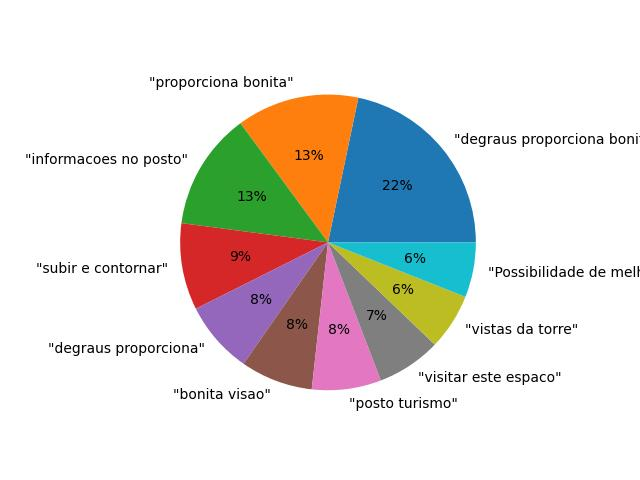
\includegraphics[width=7cm]{figuras/TripAdvisor/Activities/place0_keywords.jpeg}
    \caption{Gráfico circular gerado baseando-se nas \textit{keywords} mais usadas da plataforma \textit{TripAdvisor} referente ao Castelo de Beja}
    \label{fig:exemplofig}
    \end{figure}
    
    \begin{figure}[!htb]
    \centering
    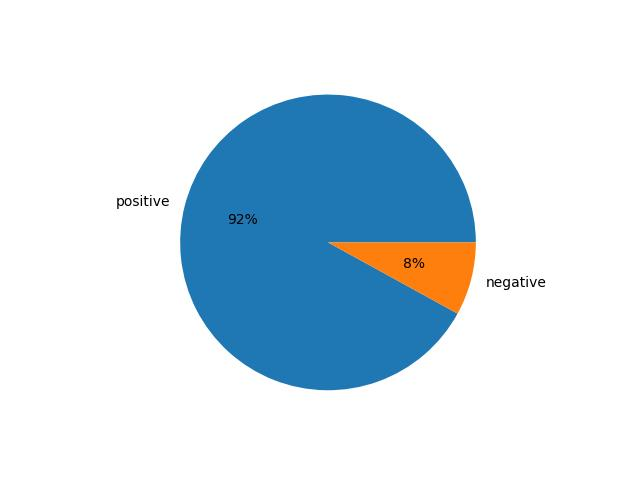
\includegraphics[width=7cm]{figuras/TripAdvisor/Activities/place8_sentiments.jpeg}
    \caption{Gráfico circular gerado baseando-se nos \textit{sentiments} mais usados da plataforma \textit{TripAdvisor} referente à Catedral de Beja}
    \label{fig:exemplofig}
    \end{figure}
    
    \begin{figure}[!htb]
    \centering
    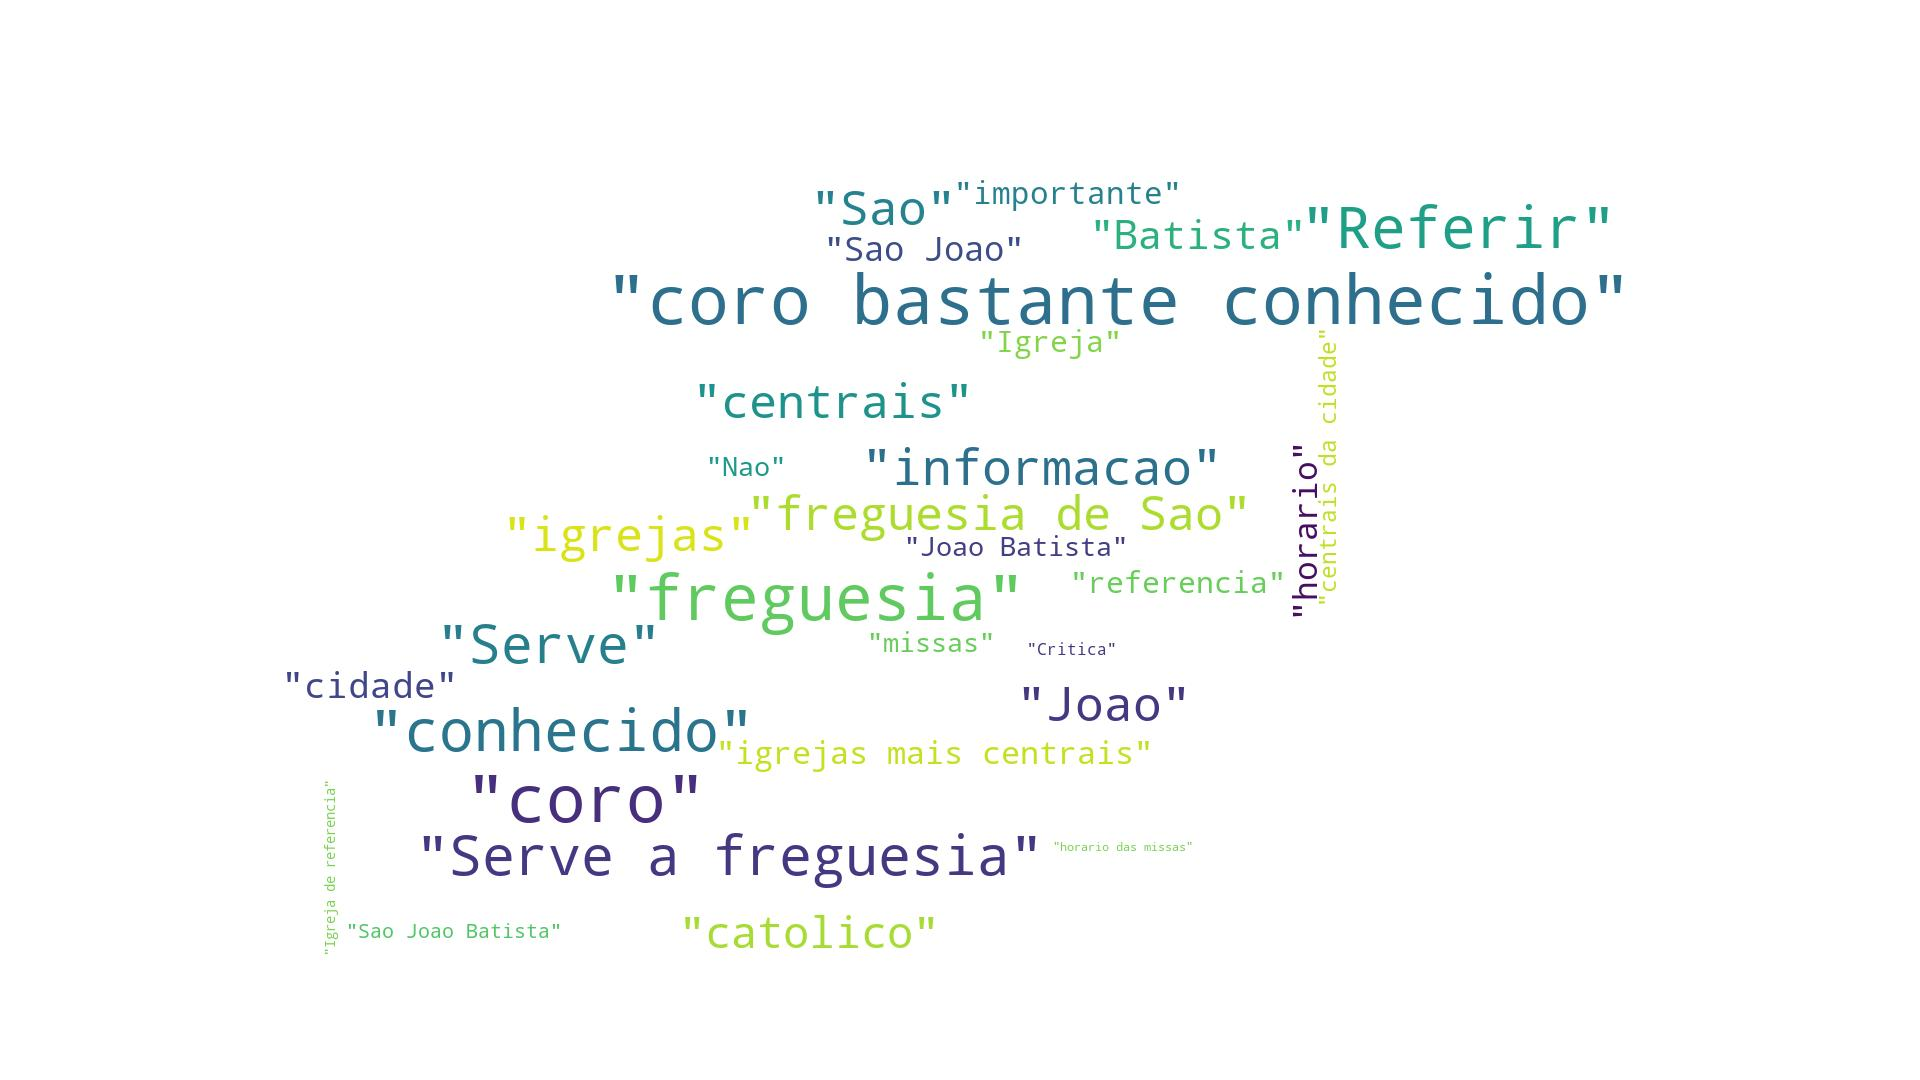
\includegraphics[width=7cm]{figuras/TripAdvisor/Activities/place8_keywordcloud.jpeg}
    \caption{Gráfico de palavras-chave e nuvens de palavras-chave contendo as \textit{keywords} mais usadas da plataforma \textit{TripAdvisor} referente à Catedral de Beja}
    \label{fig:exemplofig}
    \end{figure}
    
    \begin{figure}[!htb]
    \centering
    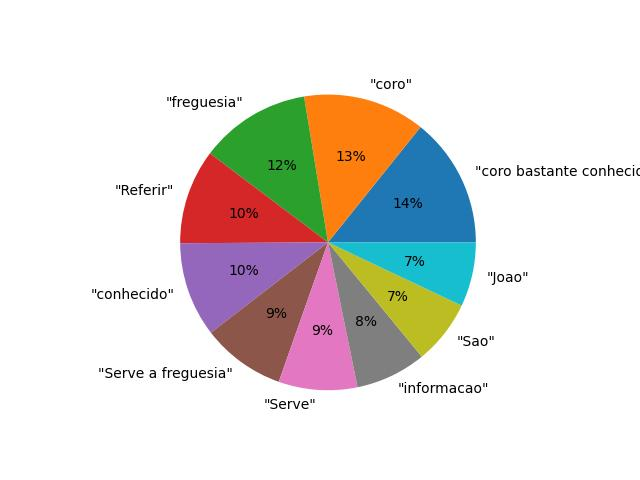
\includegraphics[width=7cm]{figuras/TripAdvisor/Activities/place8_keywords.jpeg}
    \caption{Gráfico circular gerado baseando-se nas \textit{keywords} mais usadas da plataforma \textit{TripAdvisor} referente à Catedral de Beja}
    \label{fig:exemplofig}
    \end{figure}
    
    \begin{figure}[!htb]
    \centering
    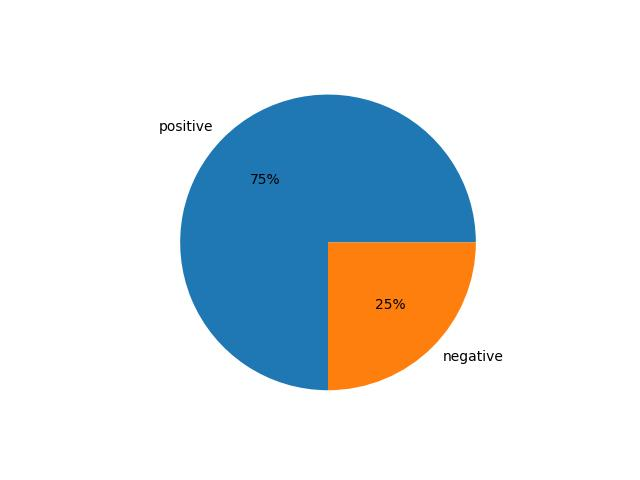
\includegraphics[width=7cm]{figuras/TripAdvisor/Activities/place21_sentiments.jpeg}
    \caption{Gráfico circular gerado baseando-se nos \textit{sentiments} mais usados da plataforma \textit{TripAdvisor} referente à Janela Manuelina}
    \label{fig:exemplofig}
    \end{figure}
    
    \begin{figure}[!htb]
    \centering
    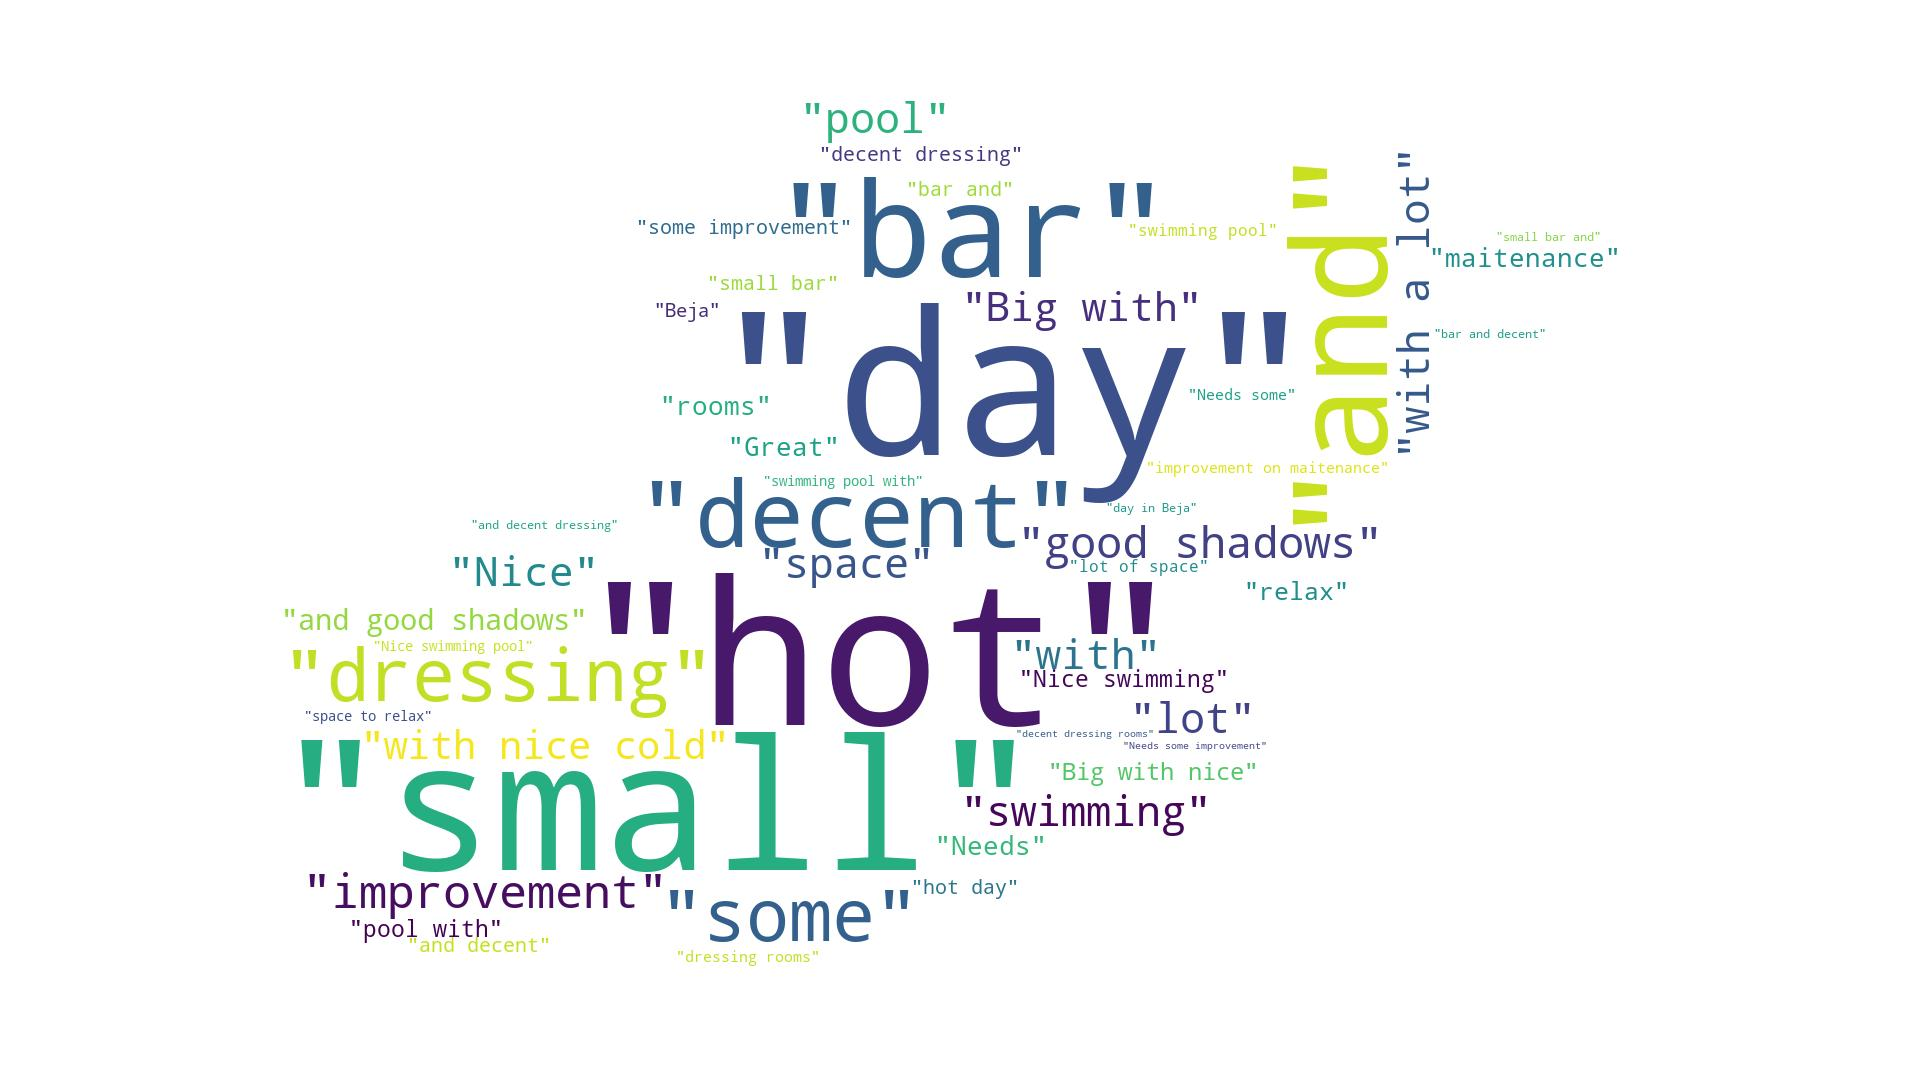
\includegraphics[width=7cm]{figuras/TripAdvisor/Activities/place21_keywordcloud.jpeg}
    \caption{Gráfico de palavras-chave e nuvens de palavras-chave contendo as \textit{keywords} mais usadas da plataforma \textit{TripAdvisor} referente à Janela Manuelina}
    \label{fig:exemplofig}
    \end{figure}
    
    \begin{figure}[!htb]
    \centering
    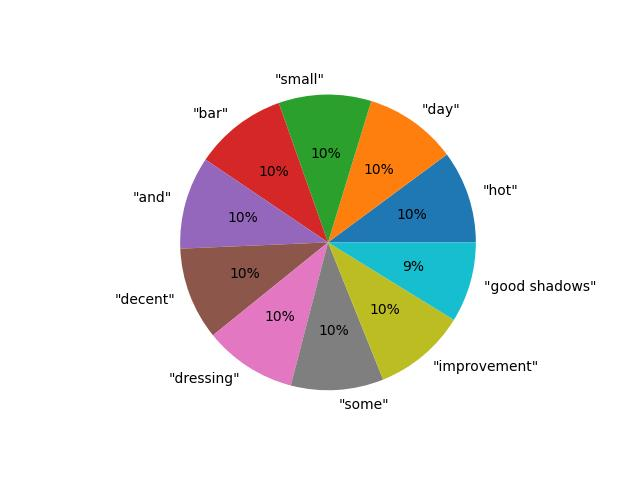
\includegraphics[width=7cm]{figuras/TripAdvisor/Activities/place21_keywords.jpeg}
    \caption{Gráfico circular gerado baseando-se nas \textit{keywords} mais usadas da plataforma \textit{TripAdvisor} referente à Janela Manuelina}
    \label{fig:exemplofig}
    \end{figure}
    
